\documentclass{sigchi}

% Use this command to override the default ACM copyright statement (e.g. for preprints).
% Consult the conference website for the camera-ready copyright statement.


%% EXAMPLE BEGIN -- HOW TO OVERRIDE THE DEFAULT COPYRIGHT STRIP -- (July 22, 2013 - Paul Baumann)
% \toappear{Permission to make digital or hard copies of all or part of this work for personal or classroom use is 	granted without fee provided that copies are not made or distributed for profit or commercial advantage and that copies bear this notice and the full citation on the first page. Copyrights for components of this work owned by others than ACM must be honored. Abstracting with credit is permitted. To copy otherwise, or republish, to post on servers or to redistribute to lists, requires prior specific permission and/or a fee. Request permissions from permissions@acm.org. \\
% {\emph{CHI'14}}, April 26--May 1, 2014, Toronto, Canada. \\
% Copyright \copyright~2014 ACM ISBN/14/04...\$15.00. \\
% DOI string from ACM form confirmation}
%% EXAMPLE END -- HOW TO OVERRIDE THE DEFAULT COPYRIGHT STRIP -- (July 22, 2013 - Paul Baumann)


% Arabic page numbers for submission.
% Remove this line to eliminate page numbers for the camera ready copy
% \pagenumbering{arabic}


% Load basic packages
\usepackage{balance}  % to better equalize the last page
\usepackage{graphics} % for EPS, load graphicx instead
\usepackage{times}    % comment if you want LaTeX's default font
\usepackage{url}      % llt: nicely formatted URLs

\usepackage{multirow}
\usepackage{ wasysym }
\usepackage{ textcomp }
\usepackage{tabularx}
\usepackage[valuemode=math,unitmode=math]{siunitx}


% llt: Define a global style for URLs, rather that the default one
\makeatletter
\def\url@leostyle{%
  \@ifundefined{selectfont}{\def\UrlFont{\sf}}{\def\UrlFont{\small\bf\ttfamily}}}
\makeatother
\urlstyle{leo}


% To make various LaTeX processors do the right thing with page size.
\def\pprw{8.5in}
\def\pprh{11in}
\special{papersize=\pprw,\pprh}
\setlength{\paperwidth}{\pprw}
\setlength{\paperheight}{\pprh}
\setlength{\pdfpagewidth}{\pprw}
\setlength{\pdfpageheight}{\pprh}

% Make sure hyperref comes last of your loaded packages,
% to give it a fighting chance of not being over-written,
% since its job is to redefine many LaTeX commands.
\usepackage[pdftex]{hyperref}
\hypersetup{
pdftitle={Ellustrate: Enabling Visual Circuit Design and Fabrication for Multimaterial Paper Circuits},
pdfauthor={LaTeX},
pdfkeywords={SIGCHI, proceedings, archival format},
bookmarksnumbered,
pdfstartview={FitH},
colorlinks,
citecolor=black,
filecolor=black,
linkcolor=black,
urlcolor=black,
breaklinks=true,
}

% create a shortcut to typeset table headings
\newcommand\tabhead[1]{\small\textbf{#1}}

% set up tight list spacing
\usepackage{enumitem} 
\setlist{nolistsep,nosep}

% for toggles
\usepackage{etoolbox}


% CHANGE FROM TOGGLE TRUE TO TOGGLE FALSE TO HIDE COMMENTS
\newtoggle{comments}
\toggletrue{comments}
% \togglefalse{comments}

% Comment region command (from Wesley Willett)
\usepackage[usenames]{color}
\usepackage[usenames,dvipsnames]{xcolor}
\iftoggle{comments} {
  %if we want to show comments
  \newcommand {\jlo}[1]{{\color{magenta}\bf{JLO: #1}\normalfont}}
  \newcommand {\cesar}[1]{{\color{NavyBlue}\bf{CAT: #1}\normalfont}}
  \newcommand {\ep}[1]{{\color{violet}\bf{EP: #1}\normalfont}}
  \newcommand {\mira}[1]{{\color{Orange}\bf{MD: #1}\normalfont}}
  \newcommand {\wil}[1]{{\color{Blue}\bf{WL: #1}\normalfont}}
  \newcommand {\danny}[1]{{\color{Red}\bf{DK: #1}\normalfont}}
}{
  %if we don't want to show comments
  \newcommand {\jlo}[1]{}
  \newcommand {\cesar}[1]{}
  \newcommand {\ep}[1]{}
  \newcommand {\mira}[1]{}
  \newcommand {\wil}[1]{}
  \newcommand {\danny}[1]{}
}

\newenvironment{myquote}{\list{}{\leftmargin=0.01\textwidth \rightmargin=0.01\textwidth}\item[]}{\endlist}
\newcommand*{\quoted}[1]{{\small{\fontfamily{cmss}\selectfont{#1}}}}
\newcommand*{\layer}[1]{{\textbf{\small{\fontfamily{cmss}\selectfont{#1}}}}}
\newcommand*{\participant}[1]{{\textbf{\small{\fontfamily{cmss}\selectfont{#1}}}}}
\newcommand*{\factor}[1]{{\textbf{\small{\fontfamily{cmss}\selectfont{#1}}}}}
\newcommand*{\nt}[1]{{\textbf{\small{\fontfamily{cmss}\selectfont{#1}}}}}
\newcommand*{\code}[1]{{\small{\fontfamily{cmss}\selectfont{#1}}}}




% End of preamble. Here it comes the document.
\begin{document}

\title{Ellustrate: Enabling Aesthetic Design and Fabrication for Multimaterial Paper Circuits}

% \title{Ellustrate: Enabling Aesthetic Design and Fabrication for Silver, Copper, and Conductive Thread Circuits}
% \title{Ellustrate: Enabling Visual Circuit Design and Fabrication for Multiple Materials}

\numberofauthors{1}
\author{
  \alignauthor Anonymized for Submission\\
    \affaddr{...}\\
    \affaddr{...}\\
    \email{...}
}
\teaser{
  \vspace{0pt}
  \centering
  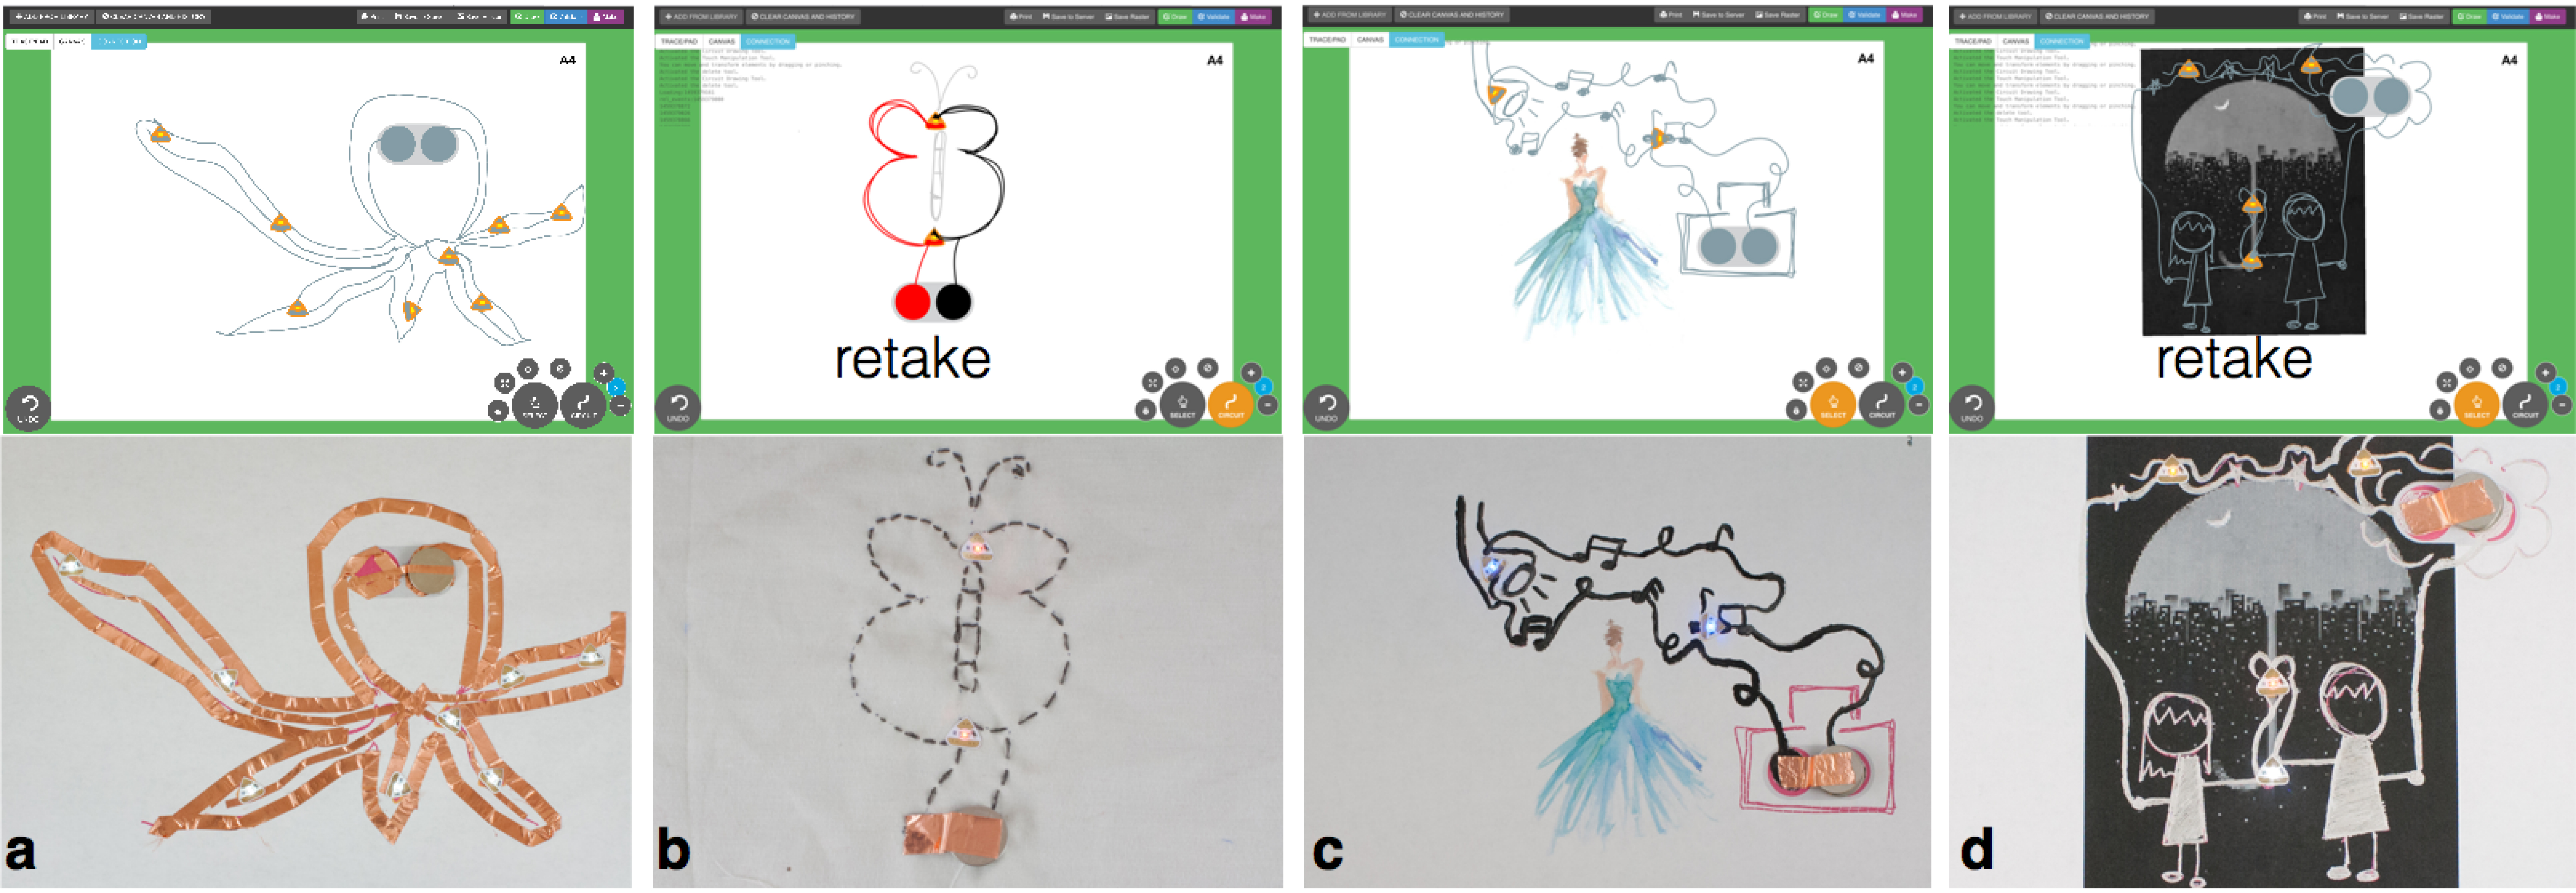
\includegraphics[width=\linewidth]{figures/Ellustrate_figures_copper_thread_silver.jpg}
  \caption{
    a) A painting made with conductive silver ink, b) a copper tape object, c) a conductive thread embroidered pattern. }
    \vspace{-8pt}
  \label{fig:teaser}
}

\maketitle

\begin{abstract}

Circuit sketching has gained traction in creative communities as a method of democratizing circuit creation, diversifying the materials and techniques used to make unique, critical artifacts. In order to support this design ecology, we present Ellustrate, a digital design tool that enables the functional and aesthetic design and fabrication of electronic circuits.
Ellustrate incorporates a holistic design cycle in a digital design tool which guides users through all essential steps towards realizing their electronic ideas. The tool provides designers with a digital assistive artboard which aids users with constructing electrically-valid circuits through a set of visual rules. Using a connectivity graph, we can provide step-by-step material-specific fabrication and debugging instructions for each design.
In a formal user study, we show how Ellustrate enables a new circuit aesthetic that operates beyond efficiency, and can serve as a scaffold for designers and artists to incorporate electronic design in their everyday practice.
We discuss how such tools that enable material-first exploration can support growing online communities. 


% and incorporates story-telling and new mental model.

% democratize electronic design to include designers and artists and examine the aesthetic value of circuit design beyond
% Ellustrate provides multi-material support and design-focused drawing tools tailored for aesthetically-driven functional circuit design. 
% Within the Ellustrate design tool, designers receive immediately feedback and corrections on their circuit design as they create their electronic artwork.
% Beyond the electrical and visual design, Ellustrate also offers step-by-step guidance on fabricating and debugging.

\end{abstract}
\keywords{
	design tool; sketching circuits; fabrication  \newline
}

\category{H.5.m.}{Information Interfaces and Presentation (e.g. HCI)}{Miscellaneous}

\section{Introduction}
Circuit design is no longer just for electrical engineers. An increasing number of crafters, artists, and designers are embedding computational circuits in everyday objects.
Once the domain of breadboards and etched copper, circuit design and prototyping has expanded to include a wide range of conductive and non-conductive materials ranging from copper tapes, conductive thread, silver ink pens, and graphite paint.
Through these materials, users are enabled to explore different form-factors across fabric, paper, and plastic.



% first proposed by Qie et al.
Circuit sketching, a fabrication process which utilizes common craft materials to create physical circuits, has become popular among makers with skills in crafting but little experience with electronics ~\cite{qi_sketching_2014, qi_stickers_2015}.
On of the greatest strengths of sketching lies in its natural and intuitive process shared by professional electrical engineers and artists alike and has large implications for early learners of electronics for empowering them to create function circuits. The sketching circuits process has shown to be increase participation of electronic design from diverse population, remove negative stigma associated with circuits, and motivate early learners. Moreover, the ability to incorporate these circuits into their own craft generates unexplored design opportunities and possibilities. 
Drawing and sketching play a critical role within the development of user interfaces. Sketching has shown to bring interesting elements to hardware prototyping, sparking creative innovations within the Maker community.
Although sketching circuit has many benefits in initial design and early electronic education, it is not explored by supported by many electrical digital design tools.


Various research fields have taken notice of the circuit sketching trend as well, creating various conductive materials (i.e silver, graphite, copper) that can be applied on paper in ways similar to a regular pen~\cite{russo2011pen}. Advances in materials have enabled a new class of circuits that are ``sketchable''. While ease of use of the conductive pen, copper tape, and conductive threads, has enabled many creative crafting projects, however, the complexity of the circuits these electronic crafts have remained stagnant. The traditional circuit design aesthetic is mostly influenced by efficiency - how to pack as many lines as possible in shortest distance from one component to another. This is an artifact of the huge demand on miniaturization of electronics and the exponentially increasing burden on electronics to conserve valuable board space. The industry-standardized interest in optimizing for speed and space have influenced early circuit education, even when optimized performance is not as big of a concern compared to eliciting interest and retaining learners.
In most circuit design tool, the final layout of the circuitalways create the straight-line, efficiency-focused, design.
Even in design tools that focus on entry-level circuit making, such as 123D Circuits and Fritzing, the functions for drawing the final printed circuit board layout still favor the traditional straight-line aesthetics.
While this tried-and-true layout method is extremely valuable, it also limits how electronics and circuits are viewed - something pedantic instead of creative. Despite the tremendous benefits brought to electronic creation and learning circuit sketching, the process has remained restricted to a physical classroom setting.


\jlo{Sketching is an integral part of design - in both visual design, and software and hardware engineering design. Digital design tools that aid in physical design have been studied extensively, and their benefits to the final physical design have been well documented. (notes to be flushed out: Material exploration - the ability to think of atoms and bits as clay - traces are not just automatic connections but of varying resistance and other properties - device physics thinking...)}

As electronic devices become more intertwined and intimate with users, the internal making of them becomes more naked and transparent. Along with the advent of structural electronics, where circuit traces and components are printed on housing of an electronic device, and wearable electronics, where electronics and active components are part of the fashion aesthetics, the ability to inject visual design into functional electronics become increasing important.

\section{Contributions}
Ellustrate aims to democratize the electronic design process to include artists and designers with no prior circuit knowledge. 
Ellustrate differs from most circuit design tools in a number of ways: a) it balances concerns of electronic validity and expressive design, b) it integrates the human back into the fabrication process, shown in prior work to improve engagement with techniques and process, and c) provides debugging assistance to aid users with correcting improperly fabricated circuits.
\cesar{+ user study}


\section{Related Work}
We looked at related work across sketching tools, physical fabrication assistance, and \cesar{BLAH}.

\begin{figure}[t]
\centering
  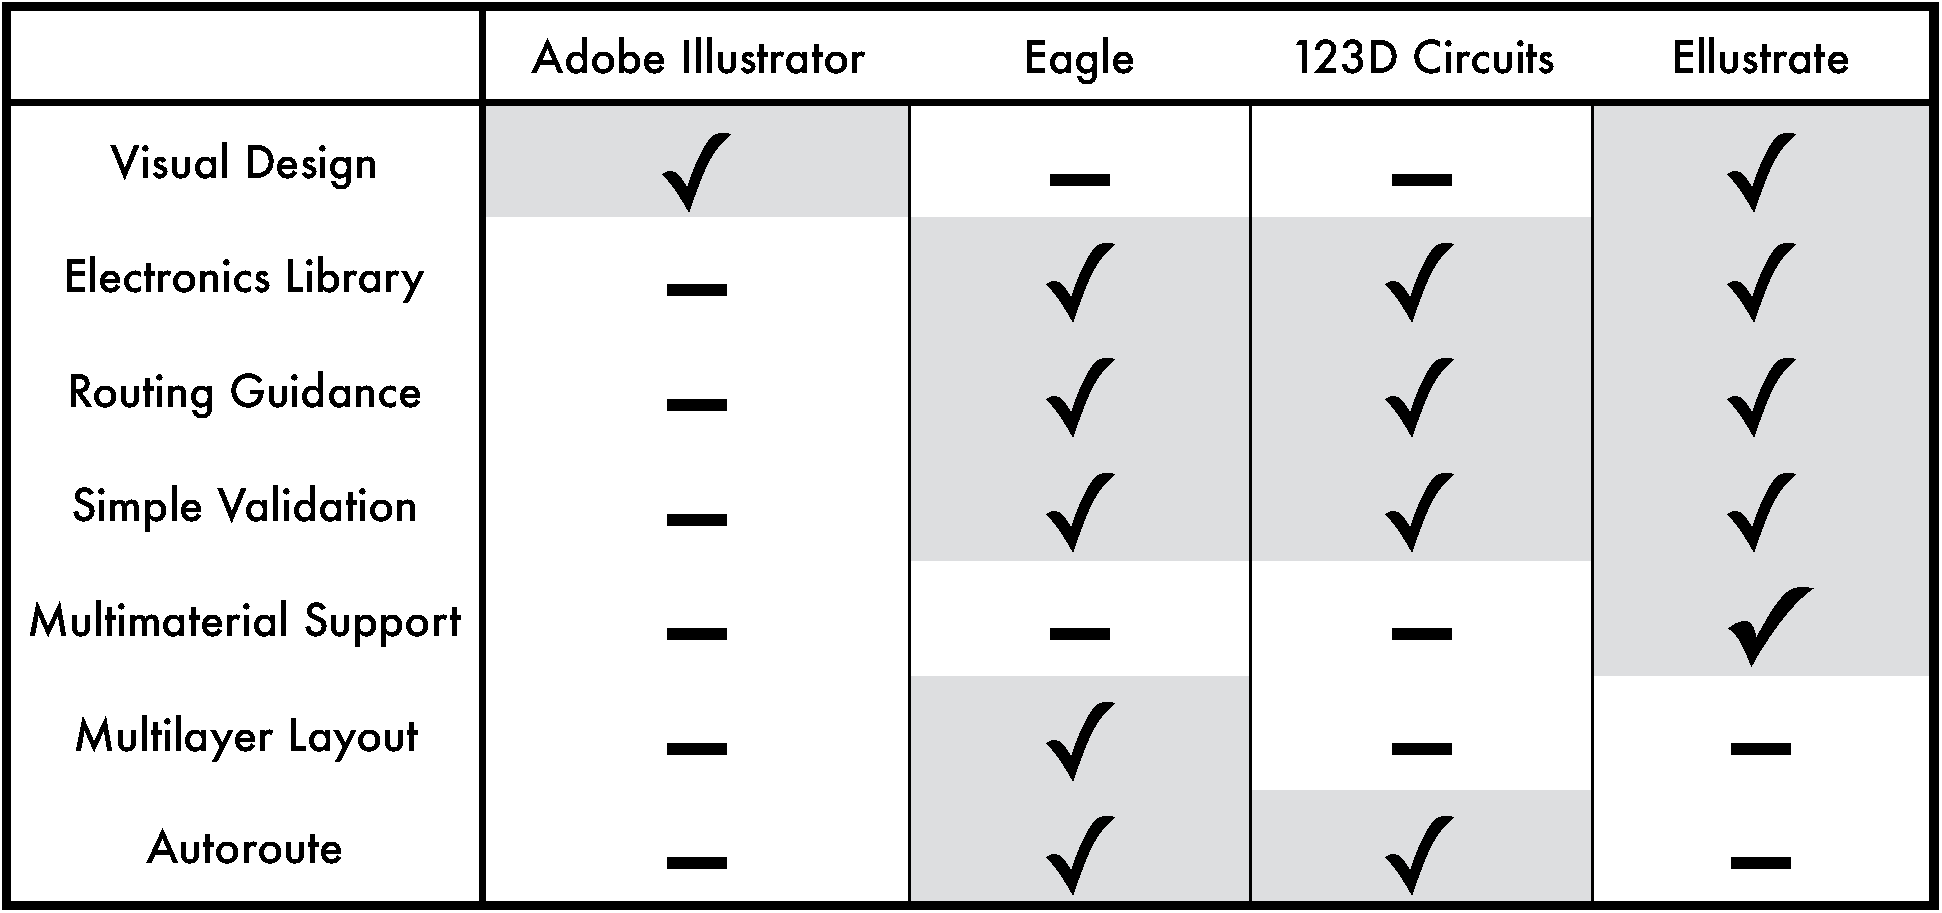
\includegraphics[width=1\columnwidth]{figures/comparative_table.pdf}
  \caption{A comparison of design tool features. Ellustrate provides coverage for both digital design and circuit design concerns. }~\label{fig:comparison_table}
  \vspace{-16pt}
\end{figure}

\subsection{Sketching Electronics on Familiar Materials}
By fabricating electronics on paper, a material that most people are familiar with, users can explore electronic design using a familiar skill set.  Augmenting such common everyday materials with power, lights, and motions has been shown to introduce a sense of wonder that resonates with people of diverse ages and backgrounds~\cite{karagozler_paper_2013}(cite Jie Qi popup book, SMA augment). Furthermore, the role of these materials in everyday life has been shown to be a natural platform for story-telling with electronics. As such, incorporating familiar materials in circuits has altered the design landscape leading to more natural, organic, and novel circuit layouts.
As more conductive and non-conductive materials develop, as does the complexity of understanding the unique electronic intricacies of each material.  Ellustrate aims to support the circuit sketching practice by providing a digital design tool that provides support for working with different materials and encourages an aesthetic exploration of circuit designs.

% Qi et al. cited the expressive medium as the main reason for the successful recruitment of a diverse population who participated in the sketching circuit workshop.
% Buechley et al. and Qi et al. expanded upon the story-telling narrative of paper circuits by leveraging sketching on paper at the onset of the creative ideation. 
% By utilizing the familiarity of a regular pencil, sketching circuits was able to combine the ideation process for both circuit and art design under one platform. (reword).  \cesar{this is too over-reaching}
 % and complement the visual design of the work.



\subsubsection{Digital Sketching Tools} 
Since sketching is such an important element of early stage design, many digital tools have been created to facilitate this process. These tools transform sketches into some form of prototype for the final design by decomposing and recognizing domain-specific symbols and lines. In SILK and SATIN, Landy et al. and Hong et al. investigate a set of software support functions for sketching user interfaces, website design, and simple logic circuits. The two tools generate a final design by ``cleaning up'' imperfections in the hand-drawn sketches - short, overlapping lines are combined, strokes are straightened, and imperfect symbols of logic gates are corrected. The traces between the elements are oftent reduced to the the shortest straight path possible. (talk about Kirchhoff pen too) With the goal of exploring the creative value in the sketches, Ellustrate does not correct or reduce the electrical traces (other than for electrical functional reasons) to maintain the sketch aesthetic. 


\subsubsection{Digital Design Tools for Physical Designs}
Digital tools offer tremendous benefits to the hardware prototyping process by allowing the user to digitally iterate a design before creating the physical version through simulations of the electric and mechanical properties. Moreover, digital tools could provide educational guidance for various aspects of the physical making process. In PaperPulse, users can connect program the behavior of a microcontroller, print out the design using a conductive ink printer, and fabricate the design with instructions provided by the tool. In d.tools, designers can design and iterate hardware interactions using microntroller and plus and play hardware (i.e. slider, LED) using statecharts. Within the AutoDesk CircuitScribe design tool, users can sketch and simulate circuit designs. The design can then be printed and a piece of paper and traced over with a silver pen. Ellustrate expands upon the aforementioned work by 1) building on a platform for tablet and stylus, thus promoting the feel of sketching within the tool, 2) augment the avaliable electronic component footprints and materials library to support a diverse sketching circuit aesthetics, and 3) integrate fabrication and debugging guidance to lower the barrier of entry for users with little circuit background.





\section{FORMATIVE INTERVIEWS}
As much as these creative forms of circuits enable early exploration of the circuit design, there are a few areas that could be improved in order to facilitate creative exploration in circuit design. In order to articulate the common difficulties that users encounter in the early stage of circuit design, we performed a series of formative user studies and interviews. 

To learn about opportunities for supporting circuit sketching and fabrication with a digital design tool, we interviewed three intro-to-circuits educators and seven potential users. 

Educators were experienced in teaching students with no prior electronic design knowledge from different domains: an intro circuits Massive Open Online Course (MOOC), Maker Faire workshops, and circuit sketching workshops. 
Potential users were recruited university students with little to no circuits background with varying level of design experience. Utilizing a think-outloud protocol, we asked interviewees to design and fabricate simple three LED\footnote{Chibitronics LED stickers} circuit with copper tape, eliciting help from the interviewer as needed. 

We discovered two major observations that informed the design of our system:

\subsection{Immediate Feedback and Validation}
\jlo{you need to describe the incident that gave you this insight.}
In hardware design, there are two main types of error that user could encounter - one is electronic design rule violations (i.e. electrical shorting), and one is functional errors (i.e. parallel LED's routed as series). They are closely analgous to the classifications of syntax and semantic errors in software. Digital tools are immensely useful when it comes to catching syntax errors, but there are few hardware design tools that provide design feedback in a way that is accessible to learners. All experts we interviewed agreed that a electrical design check as immediate feedback during the design process would greatly benefit early learners. Their opinions were well supported by exisitng literature - according to Hattie et al. and Epstein et al., providing specific immediate feedback is crucial in early learning. Although Ellustrate is not structured as a tool specific for learning, it does aim to build lasting good electrical design habits. During the circuit sketching process, we observed that the design rule that most users have trouble with was keeping track of the ground and power pads and traces and making sure that they do not short out. 

\subsection{Expert Knowledge and Guidance in Fabrication and Debugging}
\jlo{you need to describe the incident that gave you this insight.}

During our interviews, we learned that the result of the fabrication step could be most rewarding if successful, but the most demoralizing and frustrating if not. Unfortunately, assistance in fabrication and circuit debugging are not provided in most circuit design tool, and instructions in this realm remain mostly restricted to in-person classroom/workshop setting(cite Klemmer Paper-mache). We feel that providing a debugging and fabrication guide is crucial to achieving our goal of empowering designers. One major difference in fabrication that we observed in experts and entry level circuit makers was the ability to separate the circuit into small sections, and they fabricate and test each section individually in a way that minimize the chances of error propagation. We formulated expert advice into rational steps that users can follow to fabricate their design. More detailed and in depth information and debugging suggestions can be accessed as desired by the user.  
% the benefits of templates/examples in the early learning process of non-experts
% static template and their potential shortcoming 
% cite related step-by-step design tool work 



\begin{figure}
\centering
  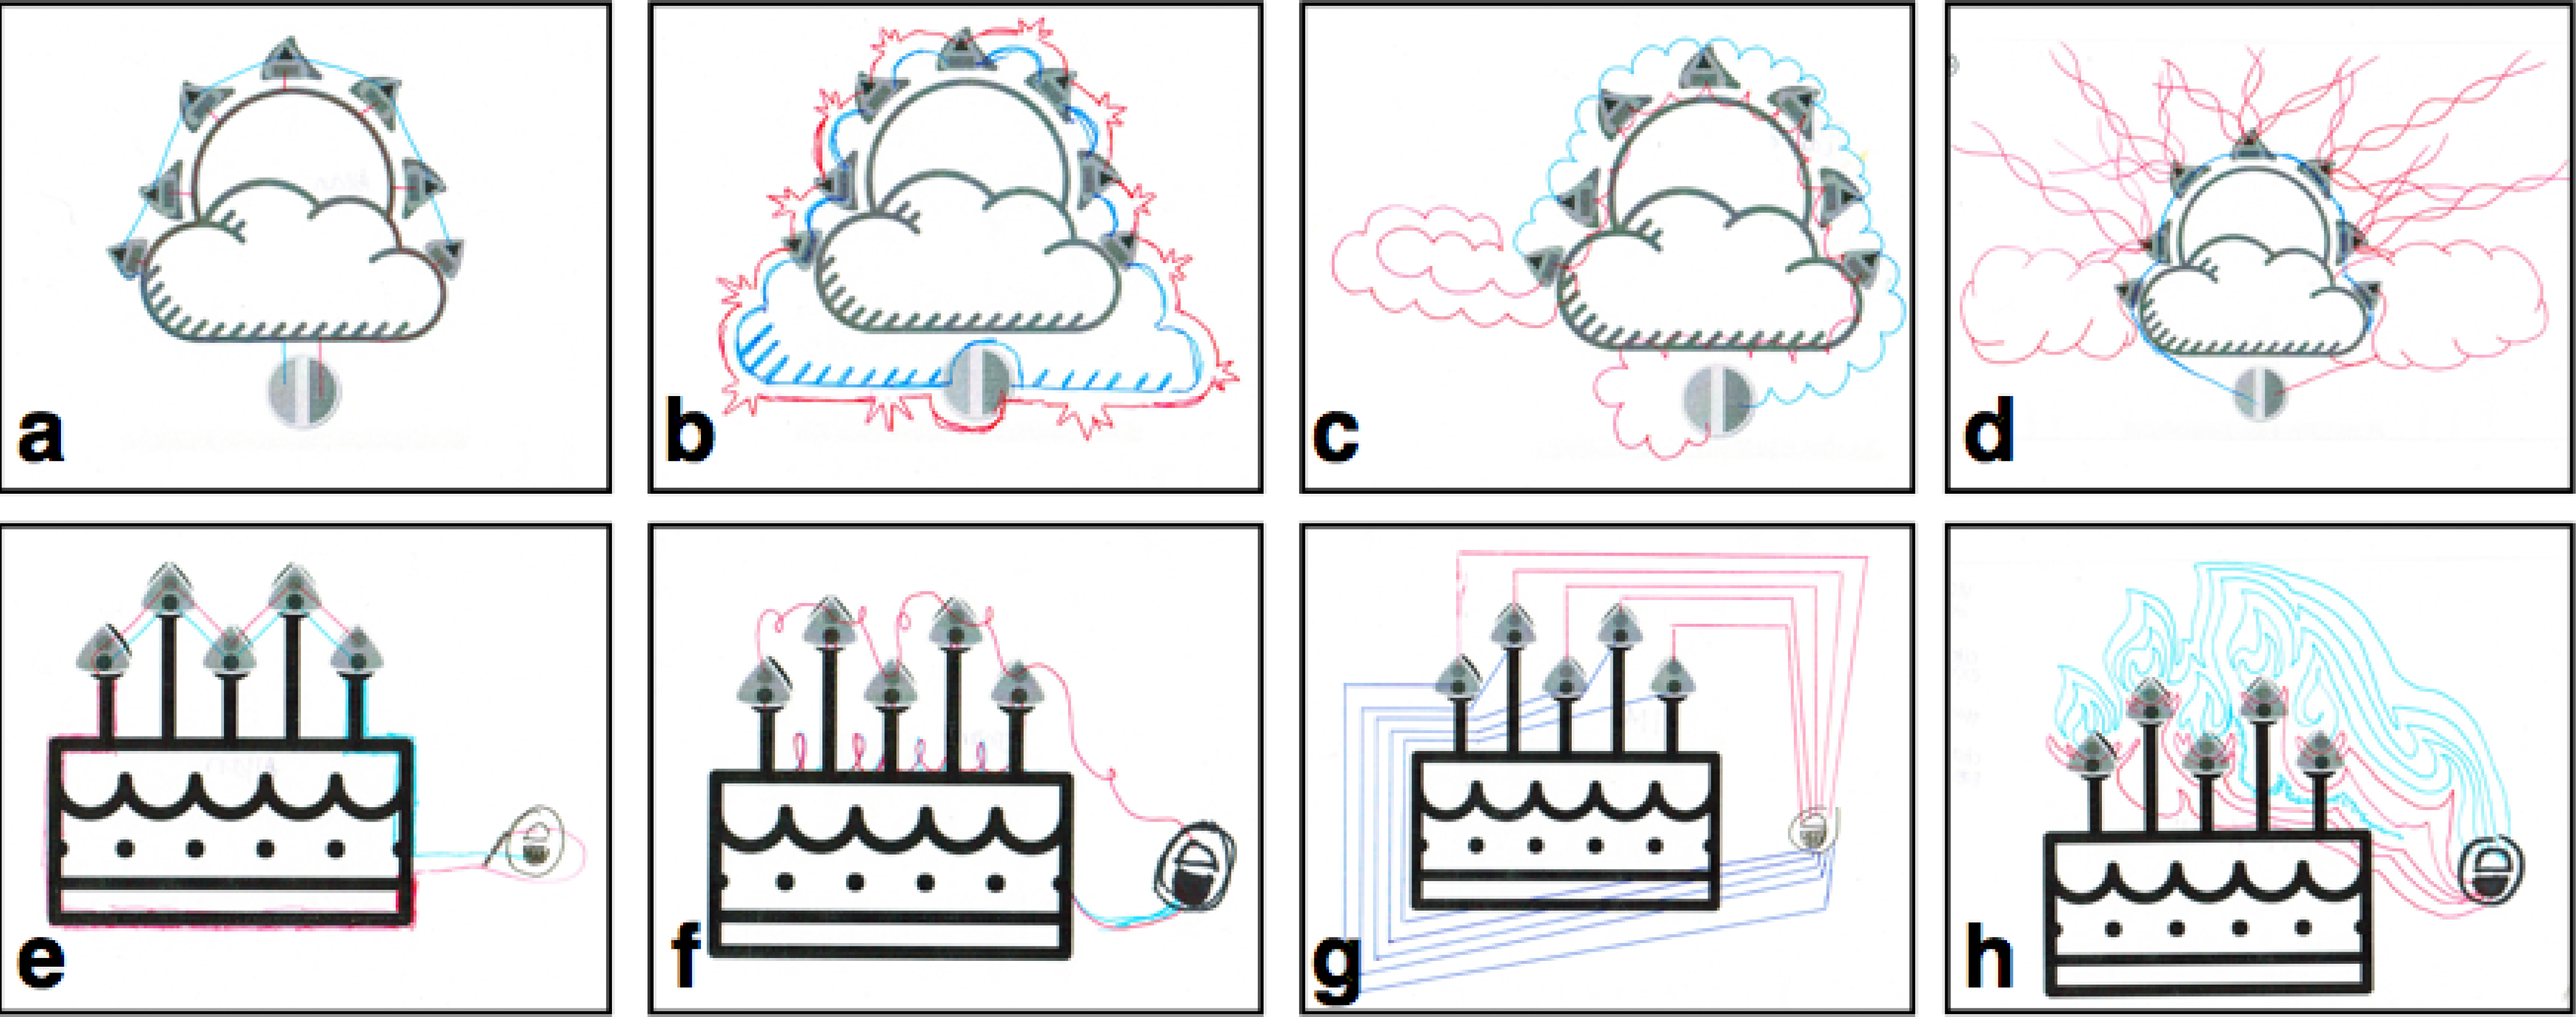
\includegraphics[width=1\columnwidth]{figures/Ellustrate_figures_formative_user_design}
  \caption{Formative user designs with pen and pencil}~\label{fig:formative_user_design}
\end{figure}

\section{Design Objectives}
Ellustrate was inspired by best practices from electrical circuit design and validation, art practice, and smart tutorial systems [peggy and mira].
These are the design objectives we set before designing our system that people should use when trying to make a good circuit sketching system. 
   \cesar{A list of circuit concerns}
    \begin{itemize}
        \item Electrical validity: Preventing shorts, forward-voltage load
        \item Legibility:
        \item Fabricability:
    \end{itemize}

    \cesar{A list of aesthetic/experience concerns}
    \begin{itemize}
        \item Craft: mechanical processes with constant interaction with the ``material" (Diderot), flow, ``Continuum of states'' (McCullough 173)
        \item Constraints as creative versus inhibatory
    \end{itemize}
And here is our attempt at doing that. 


\section{System Design}
The structure of Ellustrate follows the model-control-representation (physical and digital) (MCRpd) as proposed by Ullmer et al. Ellustrate provides a digital representation of the physical system - the circuit design and the fabrication process - and allows users to iterate their design and modify their fabrication (i.e. debug). 

The three steps in creating a circuit sketch \textendash learn basic design rules, design the circuit with incorporated visual design, and fabricate the design \textendash are dynamic processes that cannot be addressed by a static set of instructions.
We created Ellustrate, a web-based design tool that provides users with a suite of materials and components common to circuit sketching and guidance to design and fabricate a physical circuit.
The design of Ellustrate is based on a series of formative interviews, education theories, and interaction design theories \cesar{I fill that in?}.
An overview of the tool can be seen in Figure 1. Ellustrate has three design phases \textendash Design, Fabricate, and Debug \textendash representing the three stages of physical circuit creation.

Within the Design cycle, users can freely explore and sketch circuits alongside the artwork that they wish to incorporate their electronics into, with Ellustrate Design providing visual clues for electrical connections and immediate feedback for electrical design errors.
Within Ellustrate Validate cycle, the digital tool not only checks for traditional mistakes such as misplaced ground connections, but also problems that are unique to sketched circuits, such as overly long and thin traces made with the relatively less conductive crafting materials (i.e. silver, graphite, conductive threads). After the circuit design is validated, Ellustrate Fabricate mode will provide users with step-by-step instructions on fabricating the circuit and debugging problems as they arise. 


\subsection{Electronics and Materials Library}
Footprint and electronic properties (i.e. turn on voltage, maximum current) are important criteria in any circuit design. The understanding of these properties is essential to creating visually pleasing and functional circuit design. However, these vital information, which are readily avaliable in any circuit design software (i.e. Eagle, Cadence, 123D Circuits), are not avaliable in any visual design software. This greatly limits ability of the designer to create a functional circuit. In addition to the lack of electronic library, users that create physical circuits with nontraditional materials such as silver paint, graphite, and conductive thread face the difficulty fabricating traces with varying, uncharacterized, relatively high resistive materials. The problems that long, highly resistive trace often cause problems that are invisble to designers with no circuit design experience. On the BareConductive website, the manufacturer recommends users to avoid exceeding 30cm leading to a sensor due to the low conductivity. Guidance similar to this are difficult to follow during the circuit sketching process, since traces are often in non-straight lines. (...)

\subsection{Circuit Design Guidance}


Sketching circuits, especially when combine with visual design, can create complex circuit routing problems. When the electronic components are placed in a nonlinear fashion, powering all of them without shorting the circuit or creating excessively long traces become difficult. In Qi el al, a paper template is provided to workshop participants to guide them in placement of the copper tape. While this method is highly effective in aiding participants in creating a function circuits, it limits creativity in visual design (cite).  Within Ellustrate, users are encouraged to explore and iterate different placements of electronics components and traces to optimize the balance between visual design and circuit functionality. 

\subsection{Fabrication and Debugging Guidance}
The physical creation of the designed circuit is often the most difficult step in the process, as discovered in the Qi et al study ,our expert survey, and formative user study. Solving hardware problems can be In a workshop setting, guidance is provided to the participants to fabricate the circuit and debug any problems. However, in-person guidance is not easily scalable.

\section{Example Physical Circuits}

\section{Systems Details}
    As an overview, the tool was designed on an Apple iPad Pro and Pencil, chosen to best emulate a pen and paper design environment.  Ellustrate exposes to users common vector editing operations; this was intended to expose a common vocabulary to our target users, who are expected to be familiar with the vector graphics. The tool is built using the paper.js vector graphics scripting framework~\cite{lehni_paperjs_2011} and follows noun-verb drawing application conventions (e.g. click on action icon, carry out action). At a high level, the tool allows users two operations: the ability to lay down components, and the ability to make marks representing different conductive materials.

    We chose to restrict vector operations to path drawing and affine transformations of objects. This was largely motivated by an interest in reducing the tool's complexity and exposing the hand-drawn line, as opposed to ``perfect'' machine curves, to achieve a sketching-with-pen feel.

    \subsection{SVG Representation}
    All elements on the canvas were encoded as Support Vector Graphics (SVG), where the hierarchical structure was used to denote the following encoding scheme by adding a prefix to element names:
    \begin{itemize}
        \item \textbf{Ellustrate Header} (\code{EL}): Used to demarcate the topmost layers of an SVG file that should be processed.
        \item \textbf{Material channels} (e.g. \code{SI} silver-ink) At this level, the type of material used to render marks is specified. This allows for these marks to be separated easily to aid with respective fabrication techniques (similar to CMYK channel separation for offset printing).
        \item \textbf{Components} (\code{CP}) Used to specify a set of conductive elements that conceptually belong together (e.g. LED, + / – terminal, footprint).
        \item \textbf{Elementary components} \code{C(N\textbar G\textbar V)(P\textbar B), NC, C(V\textbar G)TB}.
        The N\textbar G\textbar V selector designates the accepted polarity (neutral, ground, or powered). The P\textbar B selector specifies whether the conductive element is being modeled as a path or as a blob (closed path). The TB suffix is used to mark voltage sources.
    \end{itemize}

    This representation allows us to create custom components with accurate footprints and logic specification from off-the-shelf SVG editing software. We can readily export and import representations without affecting the operation of the artwork.

    \subsection{Circuit representation}

    Once a user draws their Ellustrate circuit, we pass the design through some post-processing steps detailed below in order to extract a graph representation of the circuit:
    \begin{itemize}
        \item \textit{Decompose self-intersecting path}:  (e.g., a user has drawn a loop (l-shape) with a single stroke, then this stroke needs to be decomposed into three separate parts).
        \item \textit{Decompose intersecting path}:  (e.g. a user has drawn to paths that overlap, then these paths are split at the intersection point). Intersections are disregarded is they occur at the start or end of the path, or if the two paths in question are collinear.
        \item \textit{Blob linearization}: For each blob and intersection with a blob, we draw a line from the blob center to the inside point.
        \item \textit{Build a undirected graph}: $G$ using an adjacency list $\langle V, E \rangle$. A vertex on the graph is every start and end of each path. An edge is defined as a connection where two vertices are connected by a path or an intersection with another vertex; each edge is encoded with its material composition and cross-sectional area.
        \item \textit{Optimization step}: Vertices that are close together (e.g. four vertices at an intersection between two paths) are joined.
    \end{itemize}
    Once this graph is extracted, we use breadth-first search to find the path of least resistance \cesar{Path of least resistance is an ironic pun to Mitch Resnick's work} between two points. In order to provide a more accurate model of conductivity, we use derive a model from a set of basic electronic rules. Sheet resistance $S_r$ is the measure of resistance of thin films with uniform thickness; conductivity is modeled as the ratio of cross-sectional area and the length of the path. Thus, a path consists of a collection of edges $E$, where each edge $e$ has an associated material sheet resistivity $\rho_e$ and a sheet thickness $t_e$, which is simplified to sheet resistance $R_s = \frac{\rho_e}{t_e}$. We derive the resistance $R$ of a set of edges $E$ as:
    \begin{equation}
        R =  \sum^{E}_e R_s \int_{i=0}^{n}  \frac{1}{w_i} dl
    \label{eq:resistance}
    \end{equation}
    where $n$ is the euclidean length of an edge. Under this model, a uniform line \SI{2}{\milli\metre} thick and \SI{20}{\milli\metre} in length made with silver ink ($R_s = 0.5$) has a resistance of \SI{5}{\ohm} whereas a similar mark made with conductive thread (W = \SI{15}{\micro\metre}, $R_s = 2400$) has a resistance of \SI{1.8}{\ohm}.

    \cesar{ This would be nice to do... Traces are reduced based on resistor equivalency rules.}



\begin{figure}[t]
\centering
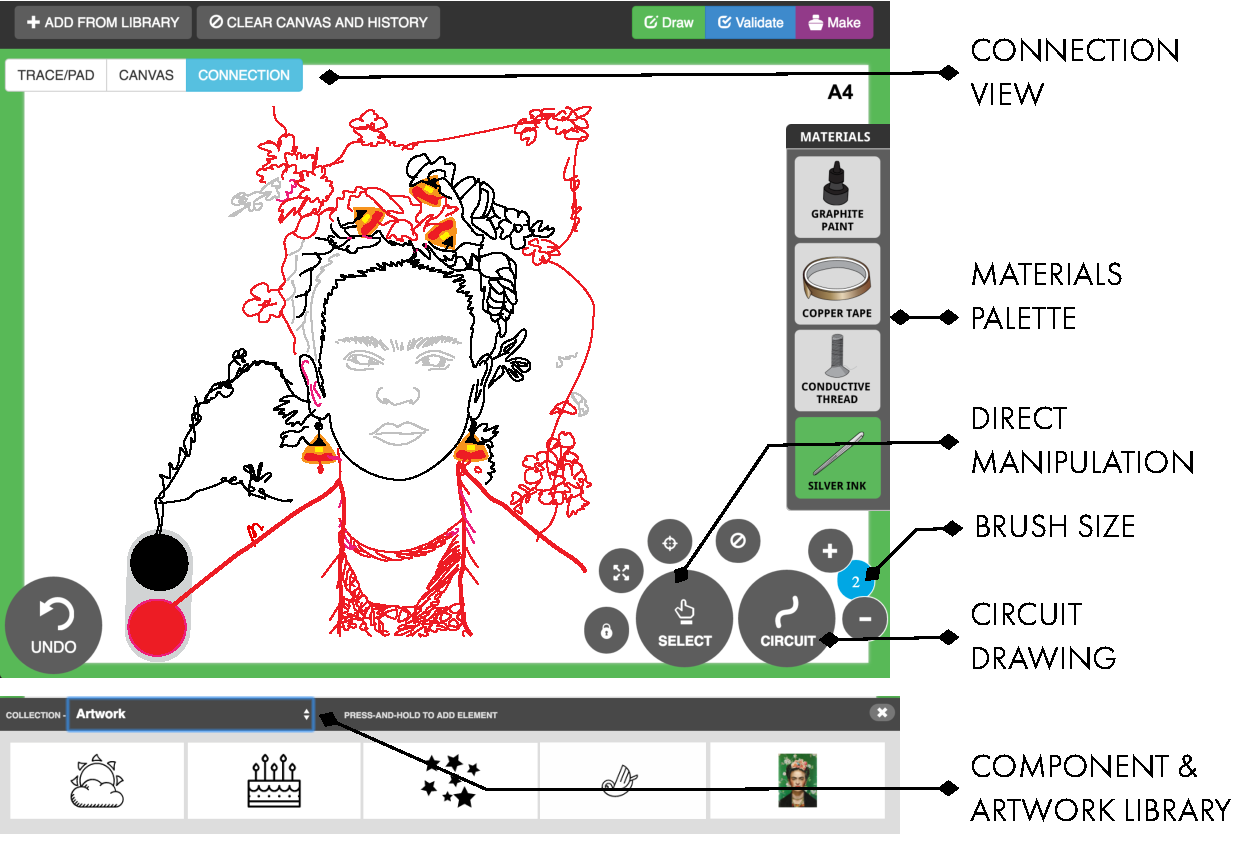
\includegraphics[width=1.0\columnwidth]{figures/designtool.pdf}
\caption{Ellustrate design tool. }
\label{fig:design_tool}
\end{figure}
\section{Digital Design Tool}
    Ellustrate aims to alter the circuit aesthetic to allow for more expressive design and fabrication of circuits, balancing visual design with circuit constraints. In this section we detail common concerns of traditional circuit design, and how Ellustrate approaches these circuit constraints.


    \subsection{The Circuit Aeshetic} Circuit design is largely concerned with created electrically valid and efficient circuits.  Due to the complexity of routing traces and the predominance of ``autotrace'' in circuit design tools, the circuit aesthetic has been largely constrained. Most notable is the rectilinear aesthetic. This is mainly an artifact of the path-planning algorithm which minimizes path length. As such, traditional circuit diagrams are minimalist in nature predominantly influenced by the the need for legibility and largely utilize patterns which reduce the cognitive load using Gestalt mechanisms. Certain design paradigms have emerged such as the power and ground rail conventions. A rail is a conductive path drawn on opposite sides of a board connected to \nt{V+} and \nt{GND} respectively. This allows for a designer to route lines without needing to exercise as much caution about causing shorts (a direct path to ground from power) by visually and physically separating offending lines. One other common visual technique is bundling, or the grouping of paths heading in the same general location. This allows for a designer to more easily trace the trajectory of a path by reducing the cognitive load of parsing the line. Non-bundled lines that are regularly spaced cause a visual experience known as as the moir\'e effect that ``shifts'' lines making it easy to lose track of one's position.

 

    \subsection{Electrical Validity}
     Circuit validation is a very large and complex field of study. In order to focus our contributions on circuit assistance design, we limit the scope of our circuit validation to deal with circuits with only LEDs, resistors, and batteries. The following design pattern can be extended to the more multi-faceted RLC (Resistance, Inductance, Capacitance) or circuits with integrated chips [Mellis].

    The most common task in electronic circuit design is the ability to connect components to sources of current. Most connections are modelled as perfect conductors, having a neglible resistance. As conductive materials enter this landscape, we encounter the need to represent the resistance or each connection (Equation \ref{eq:resistance}).

    \subsubsection{Preventing shorts}
    These connections must have an adequate resistance to prevent electrical shorts. As such, paths that originate from the voltage source (\nt{V+}) cannot make contact with paths connected to ground (\nt{GND}).

    In order to support this concern, we color-code paths, pads, and other conductive elements with different polarities as either red (positive), black (negative), or gray(neutral) and establish the following visual rule:
    \\
    \\
    \noindent\fbox{%
    \parbox{0.465\textwidth}{%
       \textbf{Visual Rule I.}
       Connections can only be made from/to similarly-colored (e.g. red\textbar red) elements or from/to neutral elements (e.g. red\textbar gray).
        }%
    }
    \\
    \\
\begin{figure}[h]
\centering
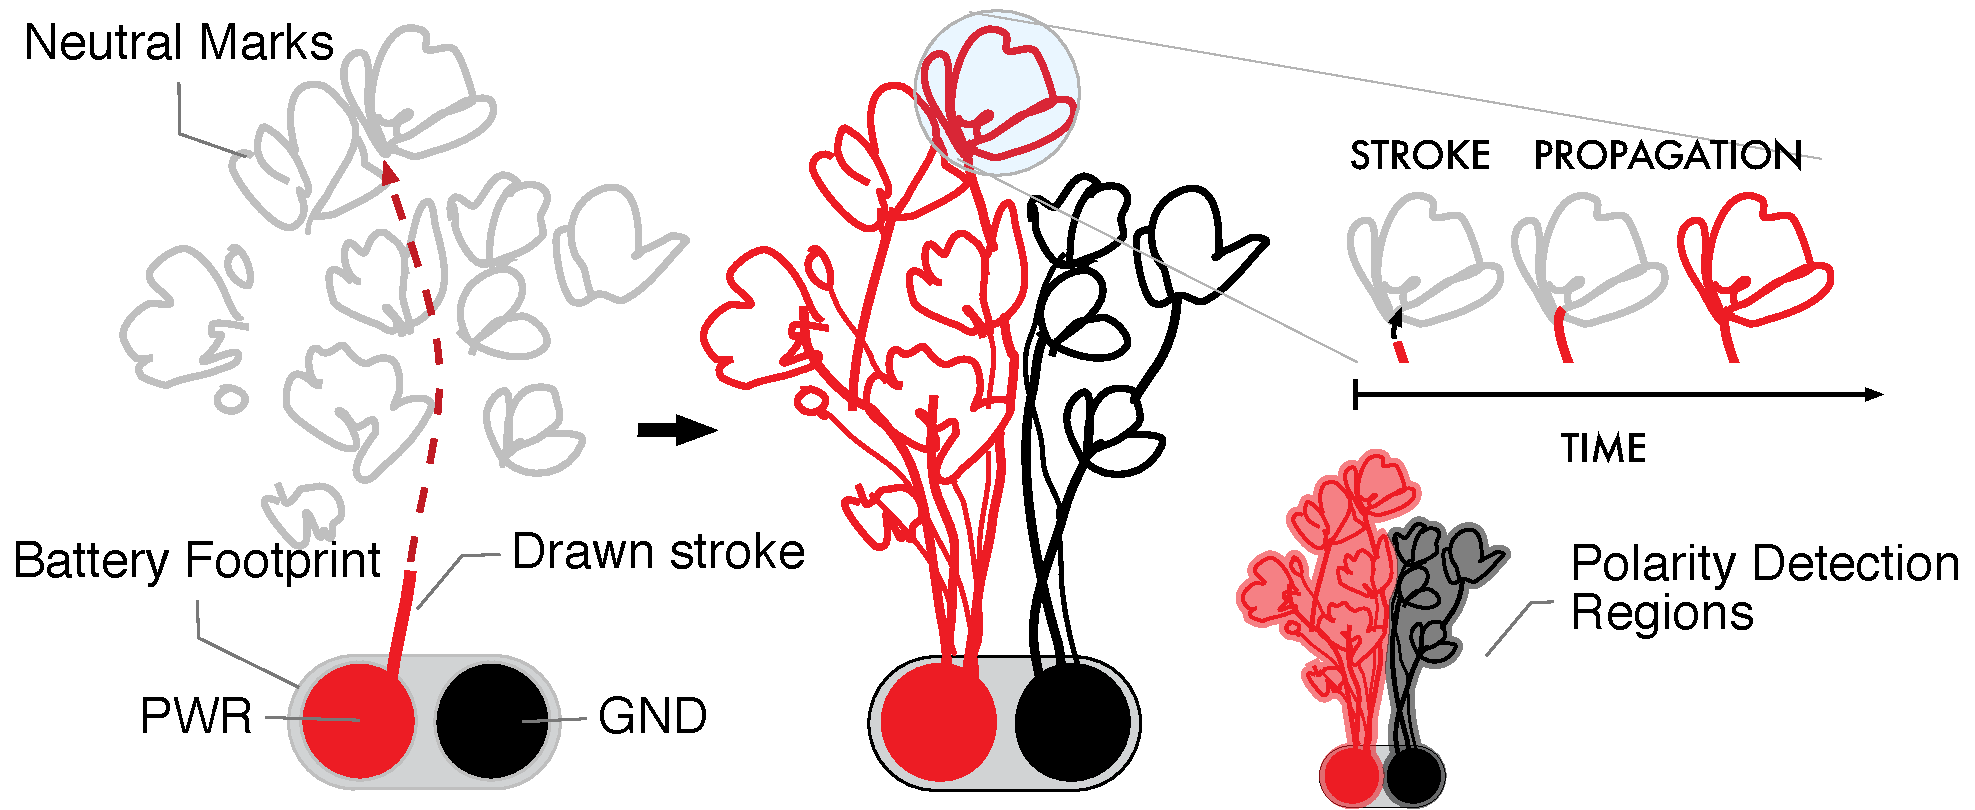
\includegraphics[width=1.0\columnwidth]{figures/propagation.pdf}
\caption{On intersection with a neutral components, path polarities update. This allows for users to design elements and then electrically incorporate them. }
\label{fig:propagation}
\end{figure}
    Should such elements cross, our tool signals offending paths to the user and are removed. If a polar connection makes contact with a neutral element, the polarity is propagated to all elements touching the neutral element (Figure \ref{fig:propagation}). This ensures that at any given time, no shorts exist within a circuit design.

    \cesar{I really want to include a visual cue for path planning, similar to the "rails" circuit design pattern. This would a) cluster terminal pads as points in a Voronoi and find the dividing line, b) use shadows of the paths to designate forbidden zones (easier to distinguish with visual desnity). }


    \noindent\fbox{%
    \parbox{0.465\textwidth}{%
       \textbf{Visual Rule II.}
       All polar elements need to be connected to its respective battery pad.
        }%
    }
    \\
    \\
    \subsection{Legibility}
        Glow relevant traces as needed.
        Connections view.
        Strip traces and show connections.

\section{Fabrication Tool}
    Once a circuit has passed digital validation, we provide a set of design-specific fabrication instructions and schematics.

    \subsection{Design schematics}
        The Ellustrate design tool outputs a to-scale version of the circuit as an SVG file. Paths are denoted with dashed lines to indicate to the user where traces should be placed. Each component footprint is also outlined. Lastly, a bill-of-materials (BOM) is produced and printable for planning and records.

    \subsection{Design-specific fabrication instructions}
        This assistance is needed to encourage best practices. It is a common trend amongst novice users to try to get to the finished product as soon as possible. This need for instant gratification can cause many fabrication errors. For instance, in a five LED circuit, it would be tempting to draw all traces and places every LED before powering on the circuit. However, a modular fabrication pattern, where one LED is placed on the circuit and verified to power on, is a tried-and-true fabrication methodology that can be used to debug circuits more efficiently. Instructions are generated by traversing the circuit tree and enumerating all possible paths to the ground node, and ordered by path length. Each path represents a modular construction. Users are instructed to first lay down the trace (with material-specific instructions e.g. silver ink needs to try, the handling of copper tape is important), laying down the component, testing for a short, and powering the circuit. These instructions can either require confirmation (does the LED turn on), or be a checkpoint (let the ink dry). In the situation that confirmation is false, a debugging tool specific to the issue. The set of debugging tools is detailed in the next section.
        \subsection{Conductive Ink Dynamic Fabrication Instructions}
        After iterations with X users, we found the following fabrication algorithm to be most effective.
        \cesar{ Joanne: Insights? Things like, why the battery first, modular decomposition, etc...}
        \cesar{ Need to add some thing about decision tree....}
        \begin{itemize}
            \item Draw the first portion of traces originating from the battery, dry.
            \item Add battery.
            \item Power Check: For each path, check that voltage greater than 3.3 V is observed.
            \item For each LED, sort by length of trace to power:
            \begin{itemize}
                \item Draw traces, dry.
                \item Check resistance of positive trace is about X ohm. If not, dry or widen.
                \item Check resistance of negative trace is about X ohm. If not, dry or widen.
                \item Place LED, pay attention to orientation.
                \item Check if LED turns on
            \end{itemize}
        \end{itemize}

    \subsection{Debugging assistance}
        In the occasion that an LED does not light up, this can likely be caused by several reasons, in order of probability.  The tool for debugging these issues is marked by parentheses.
        The trace connecting the LED to power/ground was improperly fabricated; it either contains breaks (continuity check), or the resistance is too high (ohm tool).
        An LED's orientation is incorrect (polarity check). It's cathode and anode where placed on opposite traces.
        The LED component is not making proper contact with the sheet (ohm tool).
        An LED is defective.
        The battery has lost charge.

        The following modules describe the input circuit description for the generating specific debug instructions.

        Continuity check
        A continuity issue results when a trace is not fabricated correctly; a break in this trace will result in an interrupted connection preventing the flow of electricity. This tool feature informs the user where to start and end, checking continuity be moving the lead on a multimeter (set in continuity detection mode) along the length of relevant traces.

        Polarity check
        A user is provided with this template circuit which connects two traces to the a battery. A user can place the component of interest, such as an LED, and check the polarity of the component by placing it on the traces and observing changes in behavior. Should a user experience a non-working LED, they are encouraged to verify that the orientation of the LED be correct. Although we don't foresee these issues being of major concern since LEDs are housed in perceptually-identifiable packages, we recognize polarity being a common issue and provide a simple tool to address it.




\section{EVALUATION}
    Here we describe an overview of our formal user study. The goal of this study was to conduct a usability evaluation of the tool, specifically observing at how circuit design contraints influence the visual aesthetic and how fabrication assistance influences agency. 

\subsection{Participants}
    We recruited 10 participants (avg. 28 years, 7F, 3M) well-versed in visual design, but with no prior experience with circuit design. Proficiency was self-reported in a preliminary survey. Participants were recruited from a mailing list of Architecture, Art, and Design students at our institution and from the surrounding community via Craigslist.

\subsection{Materials}
    We constrained our evaluation to a single circuit building material --- silver ink was chosen due to it's user-friendly pen form factor to have analogous tangible input with the Apple Pencil. For the study, our electronics library was constrained to fixed set of finger-sized manipulatives: $<= 5$ Chibitronics LED stickers, and a single CR2032 coin-cell battery.We also exposed a set of SVG graphics with different layout compositions (figurative, linear, radial, and random placement) in order to evaluate how users navigate circuit rules with spatial constraints. 

\subsection{Study Design}
    Each participant was invited to individually meet with us in our studio space. Participants were paid \$20/hr; each session lasted two hours and consisted of a warm-up tutorial, a digital design task, a physical hand-fabrication task. We also conducted interviews before and after each session. Participants were also asked to reflect out-loud their reflections on tools and design process, specifically vocalizing their design choices and shifts, as they went through the workshop. Due to the visual complexity of the circuits, the experimenters aided with interface and fabrication issues when they arose. We report such occurrences for future work to support a larger corpus of visual styles. 

    % power requirements
    \textit{Warmup}. We provided praticipants with relevant background information for understanding the primary concerns of circuit design and building. A brief introduction covered electricity basics (voltage, resistance, and current using the water metaphor ~\cite{gentner_flowing_1982}), polarity (e.g. preventing shorts, directionality of components), and operation of equipment (laying traces with a silver ink pen, resistance and voltage checks with a multimeter). To ground the concepts, participants were guided by the researcher in fabricating a simple, one-LED circuit powered by a coin-cell battery. Tutorial material was available as reference throughout the study. 

    \textit{Design Task}. Participants were then given a design task to design a circuit with any or all of the available materials for a period of \cesar{BLAH}.  Participants were then shown the validation of their circuit. If there were issues, they were asked to attempt to fix and iterate on their circuit design. 

    \textit{Fabrication Task}. Once successfully validated, our system produced fabrication instructions. A to-scale schematic was printed. Users were asked to fabricate their circuits. They were given \cesar{BLAH} time to complete the task.  


\subsection{Metrics}
    \jasper{Justification for metrics goes here.} We asked participants to rate their experience with the tool using five-point semantically anchored Likert questions (1=Strongly Disagree, 5=Strongly Agree):
    \begin{itemize}
      \item \factor{ASSISTANCE (As)}: The tool has helped my physical circuit debugging process.
      \item \factor{AGENCY PRE- (pA)}: I feel capable of fabricating a circuit like this before using the tool.
      \item \factor{AGENCY POST- WITH TOOL (ApT)}: I feel capable of fabricating a circuit like this after using the tool with the tool.
      \item \factor{AGENCY POST- WITHOUT TOOL (Ap)}: I feel capable of fabricating a circuit like this after using the tool without the tool.
    \end{itemize}
    In particular,  \factor{AGENCY POST- (WITH TOOL)} describes the subject's experience of designing a circuit specifically with Ellustrate, while
    \factor{AGENCY POST- (WITHOUT TOOL)} generalizes how Ellustrate may serve as an educational tool.


% \subsection{Other evaluation not done}
% (might add: Additionally, 10 participants from technical fields (i.e. computer sciences, mechanical engineering, material sciences) who had little to no prior experience with circuit design were recruited. Experience with circuit design was determined from self-reported feedback. Participants were recruited from a mailing list of technical departments.)% Participants were given a bunch of funky circuits: continuity trace issues, component connection issues, and polarity issues. They were asked to debug the circuits using our tool and without our tool. We timed the amount of time it took them to figure the problem out and fix it.



\begin{figure}
\centering
  \includegraphics[width=1\columnwidth]{figures/Ellustrate_figures_Users_in_action}
  \caption{Users designing and fabricating their circuits with Ellustrate}~\label{fig:users-in-action}
\end{figure}


\begin{figure}
\centering
  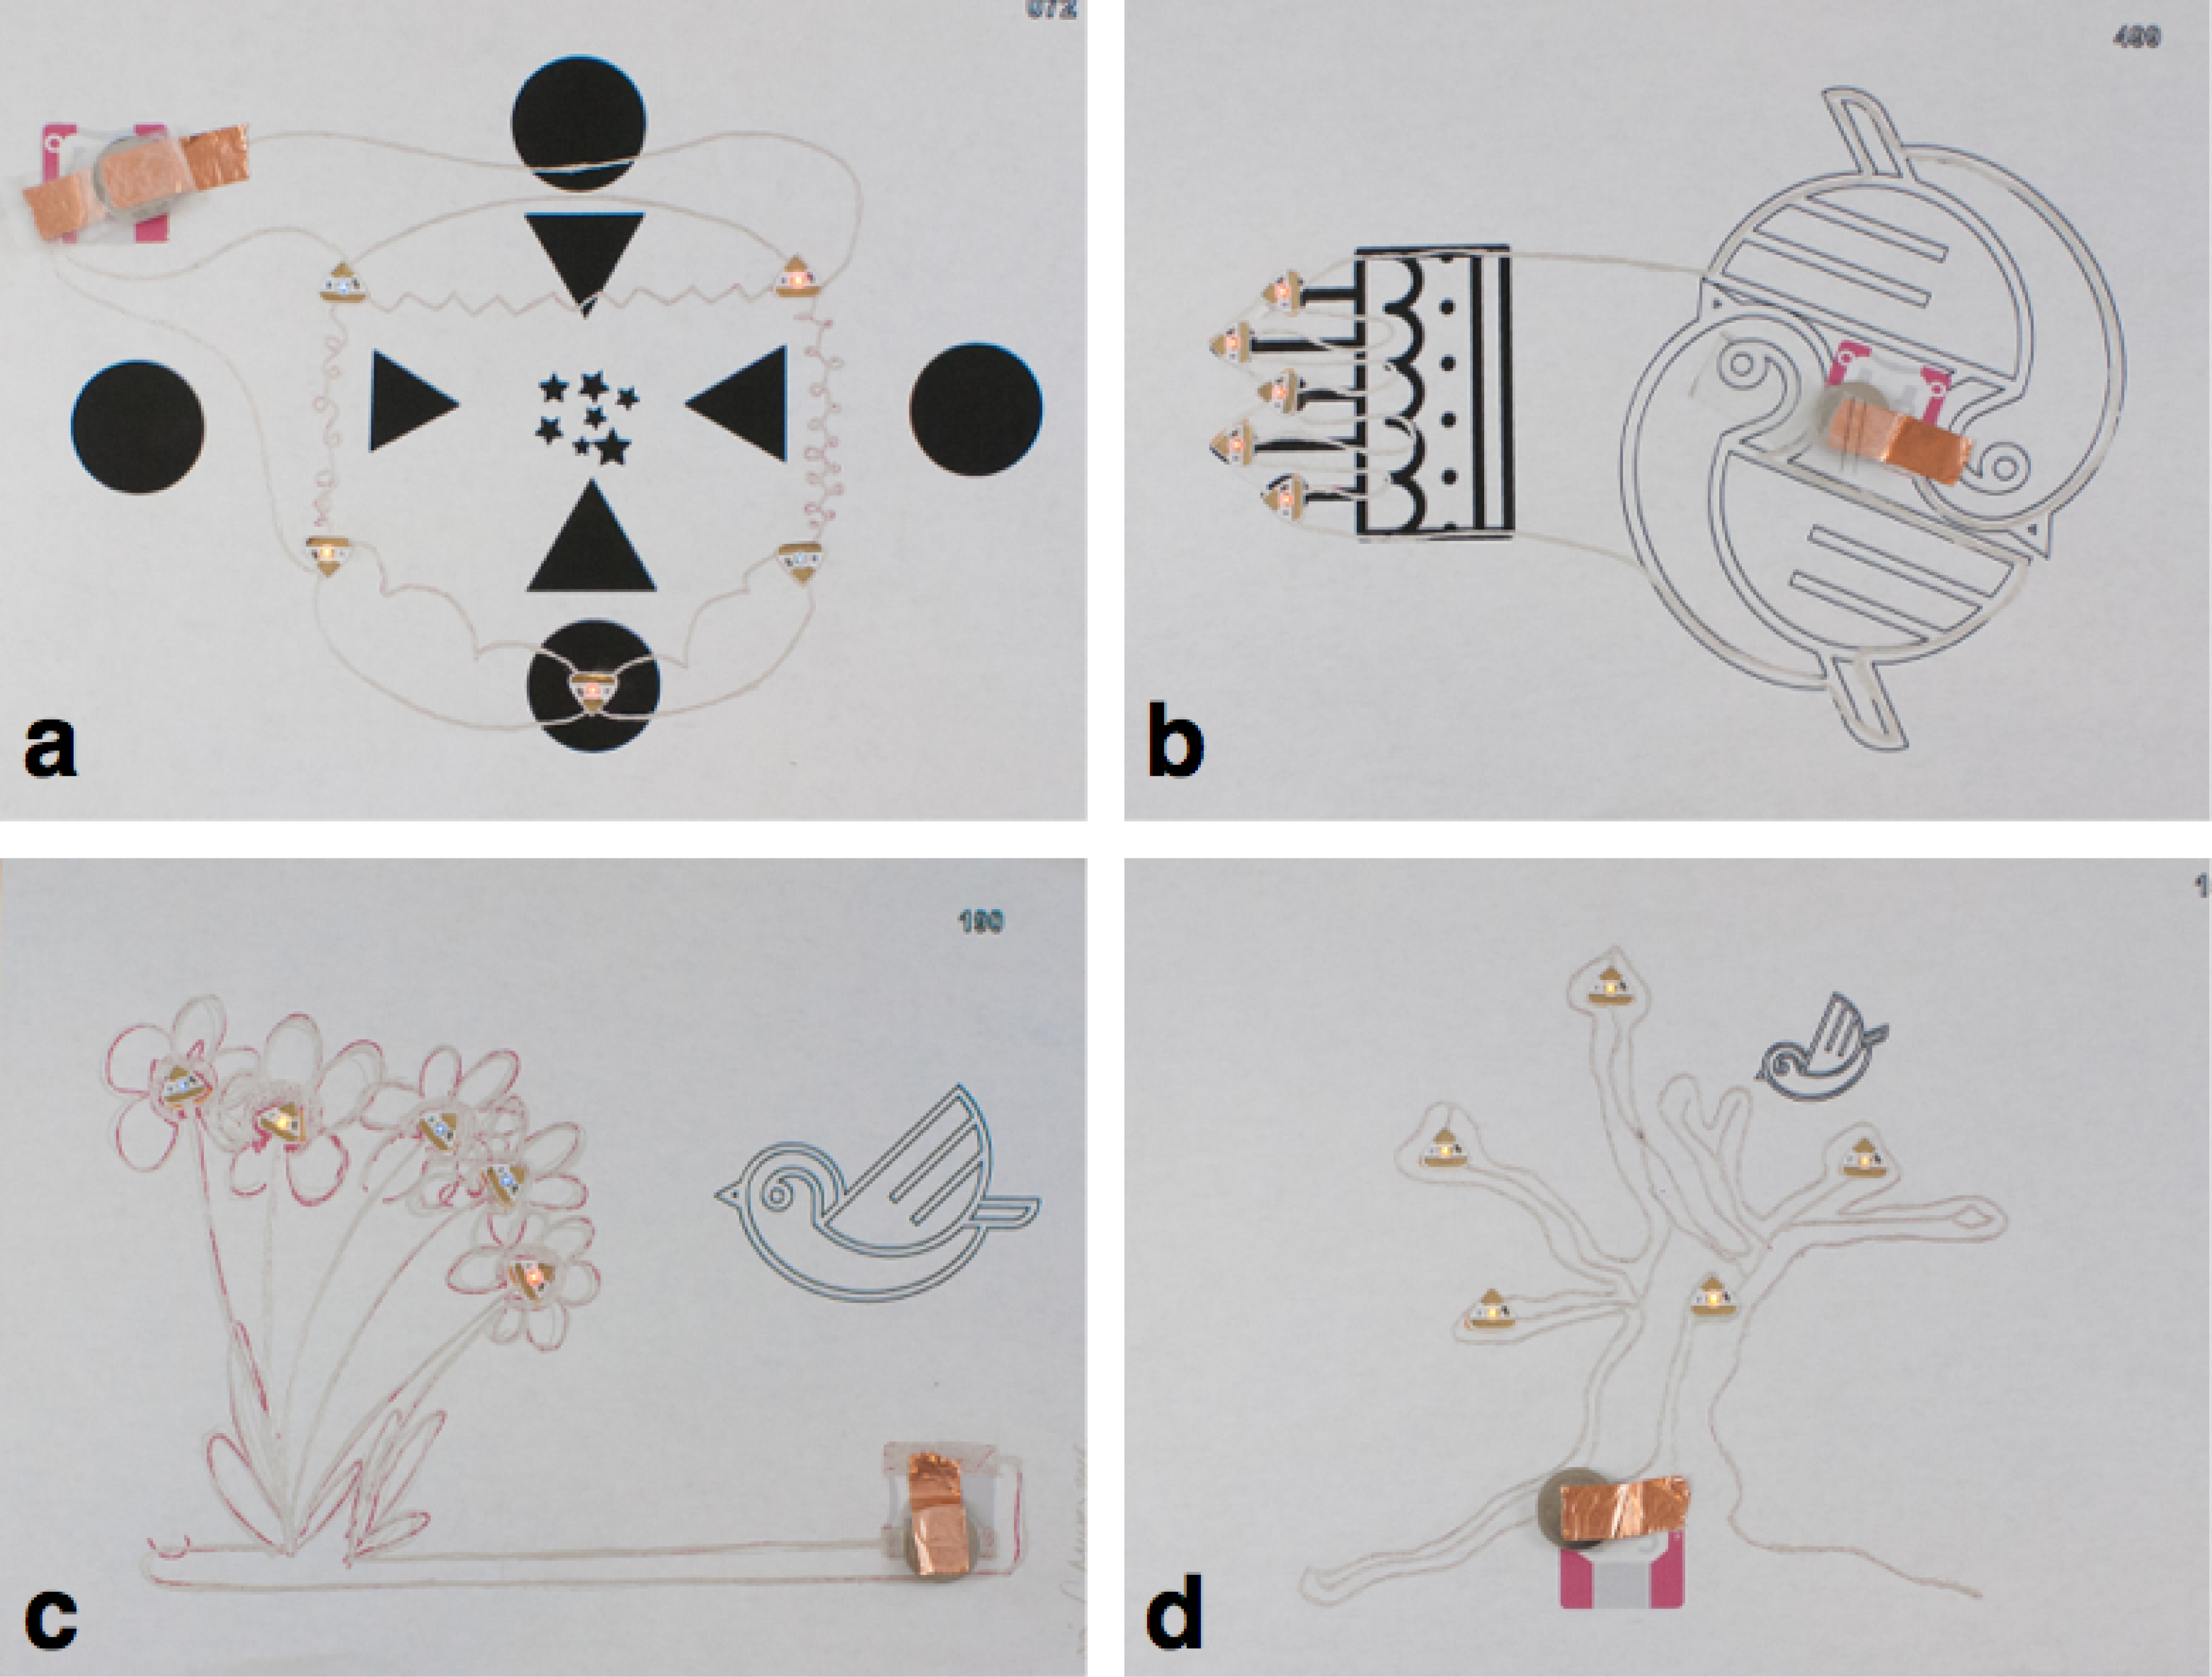
\includegraphics[width=1\columnwidth]{figures/Ellustrate_figures_Users_artwork}
  \caption{Sketched circuits made by users}~\label{fig:user-artwork}
\end{figure}




\begin{figure}[t]
\centering
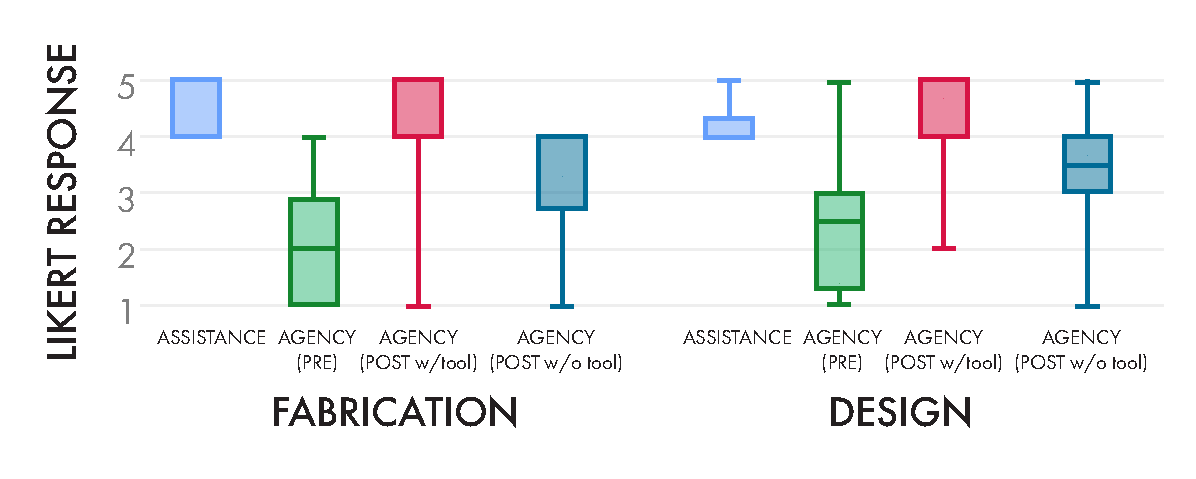
\includegraphics[width=1.0\columnwidth]{charts/boxplots_quant.pdf}
\caption{Results from fab tool and design tool. }
\label{fig:fab_tool_results}
\end{figure}

% \begin{figure}[h]
% \centering
% 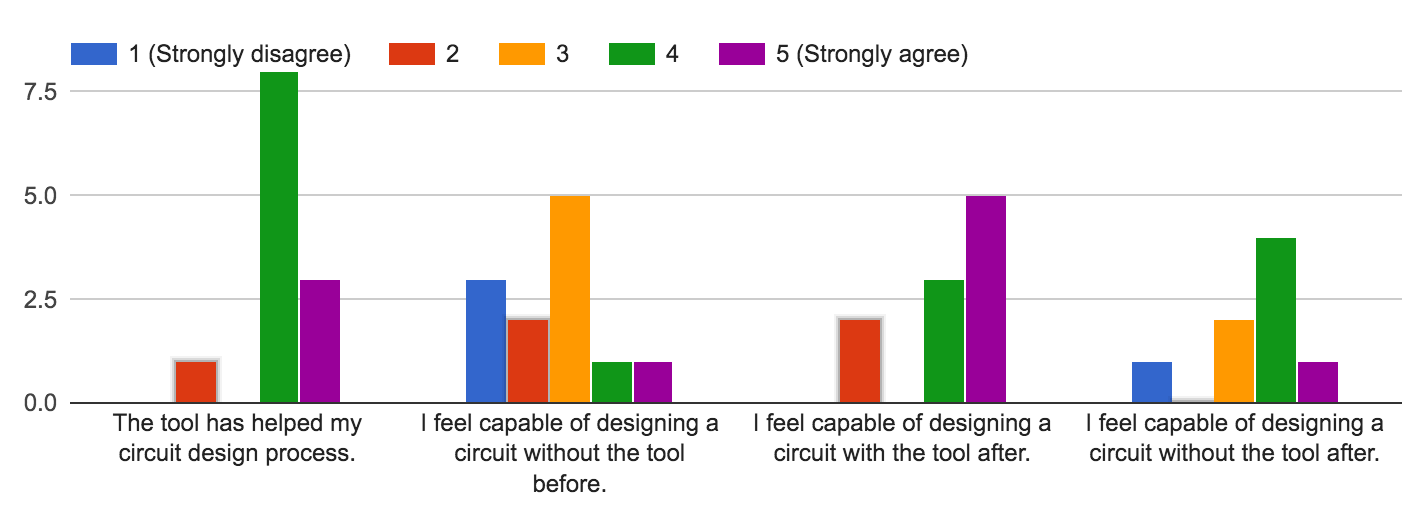
\includegraphics[width=1.0\columnwidth]{figures/design_tool_results.png}
% \caption{Results from design too. }
% \label{fig:design_tool_results}
% \end{figure}
\section{Results}
  % For the design step, participants generally viewed the tool as useful, reporting a \factor{ASSISTANCE} of $4.2 \pm 0.42$. 
  % The data suggest that the tool increased participants' agency in designing a paper circuit.  in constructi \factor{AGENCY PRE-} of $2.4 \pm 1.26$ 


  % and found increased agencies after using the tool. Participants self-reported an \factor{AGENCY POST- (WITH TOOL)} of $4.0 \pm 1.22$ 
\cesar{Overview goes here} 
All participants successfully completed their designs; some designs are represented here in Figure \ref{fig:user-artwork}. 
We first report quantitative results and then discuss interview responses in the context of specific observations and insights from the study.

\subsection{Quantitative Analysis}
  At the onset, participants expressed uncertainty and apprehension when asked to produce a visual circuit design (\factor{A} $2.4 \pm 1.26$), specifically noting \cesar{the large amount of information presented to them created a large cognitive block to what they were going to draw}
  \begin{myquote}
   \vspace{-2pt}
    \participant{Participant \#???}:
    \quoted{ I wish I could say I could make that circuit. But with all those constraints, its hard for me to even think creatively. I'd rather try to make a simple circuit, get that working, and alter my design little by little from my known threshold of skill.}
    \vspace{-2pt}
  \end{myquote}
  \cesar{Jasper: verify the below}
  All participants reported feeling that the design interface assisted them in creating the design (\factor{A} $4.2 \pm 0.42$). They felt the assistance non-intruding, citing the visual rules as fun and interesting. Many participants expressed that they wanted to design using the black and red as design elements in their visual compositions and noted that the constraint of color opened their compositions to be more explorative. 
    \begin{myquote}
   \vspace{-2pt}
    \participant{Participant \#???}:
    \quoted{ I know that the red and black are electrically important, but I just like how they look in my composition.}
    \vspace{-2pt}
  \end{myquote}
  Participants expressed a heightened caution from accidentally overlapping colored paths; few participants triggered the warning. Those who did expressed surprise and immediate recognition of their error. 
  \begin{myquote}
   \vspace{-2pt}
    \participant{Participant \#???}:
    \quoted{ I dozed off, but its okay. I know exactly what I did wrong; I realize I have to keep these elements on separate sides of the page. It causes my to think and plan, but I find that interesting and stimulating.}
    \vspace{-2pt}
  \end{myquote}
  All participants felt that with the tool, they feel empowered to visually create their own circuits (\factor{ApT} $4.0 \pm 1.22$). Several expressed agency to even create designs without the tool (\factor{Ap} of $3.4 \pm 1.27$), noting the simple coloring scheme as the most valuable in aiding their visual design practice. However, several noted that the digital form factor, although more fluid than expected, left much to be desired from pen and paper, citing resolution and accidental markings (from digital artifacts). 

  \cesar{Some note about validation and them going back to fix designs. Insert fatal errors here. People are too *** creative.... Number of vertices on a design was v= 10000000, compared to its stale circuit equivalent of v=8, e=30. Optimization steps need to be taken to prune the electrical tree during drawing time. }

  Participants expressed a much larger difference with the fabrication tool. Although in a familiar form factor, users still expressed hesitation (\factor{pA} $2.1 \pm 1.2$) especially with regards to understanding when to use the multimeter. The fabrication tool provided for them with much needed guidance; participants felt highly assisted with the tool $\factor{A} 4.4 \pm 0.52$. Many expressed that their own construction patterns were completely different from the tools suggestions
  \begin{myquote}
   \vspace{-2pt}
    \participant{Participant \#???}:
    \quoted{I had no idea where to begin! As I was doing the steps, I realize I would have gone about this totally differently. }
    \vspace{-2pt}
  \end{myquote}
  The most common intended fabrication process was laying out the traces, then adding the components. 
  However, as they moved through the fabrication steps, all participants detected the pattern and after practice with the modular decomposition, likened it to a ritual, mechanic repetition of the hands that they experience when in their respective crafts.
  \begin{myquote}
   \vspace{-2pt}
    \participant{Participant \#???}:
    \quoted{I started seeing the pattern and the intention behind the steps. Putting the battery first allows me to not have to worry about power as a variable. Drawing modularly the electric lines makes it much more likely that I will succeed.}
    \vspace{-2pt}
  \end{myquote}
  Many reported the modular lighting of LEDs as motivation to keep on continuing; there was a general consensus that more fanfare was needed. 

  \begin{myquote}
   \vspace{-2pt}
    \participant{Participant \#???}:
    \quoted{ Once I got the first light to turn on, I knew I could complete the circuit. Each light was like a little treat. Upon running into a problem, I felt confident that I could solve the issue.}
    \vspace{-2pt}
  \end{myquote}

  At the same time, we noted differences within the role of the tool. One participant found the construction initially useful, but once they learned the process they felt that it was simple to replicate on their own (\factor{Ap} $3.3 \pm 1.3$).   They noted that the multimeter operation was intimidating, but after using it, they felt it was greatly helped in revealing what was happening with the circuit. They expressed an interest to be able to ``dive deeper'' into the reasoning and the logic behind the steps and how the internal circuit is operating. The most valuable feature of the fabrication tool was the visual highlighting of paths and a feeling of being guaranteed a success (\factor{ApT} $4 \pm 1.7$). 

  \begin{myquote}
   \vspace{-2pt}
    \participant{Participant \#???}:
    \quoted{ Whoa. I realize my circuit is super complex. I'd hate to spend all this time drawing my detailed illustration and not know which line is important to the circuit. When I clicked this [highlighting of the path], it takes away that need for me to visually trace the path to the battery. }
    \vspace{-2pt}
  \end{myquote}




  % Given an overall \factor{AGENCY PRE-} of , we observed an increase in agency after using the tool with an \factor{AGENCY POST- (WITH TOOL)} of $4 \pm 1.73$ and an 
% 
  % In both the fabrication and design steps, we observe strong increases in both agency metrics, suggesting that the tool successfully enabled users with various backgrounds in circuit design to create circuits with a high degree of agency.
  
  % \jasper{More quantitative analysis needed?}
\subsection{Analysis of Users' Designs}
  Participants' designs demonstrate how users balanced electrical requirements with aesthetic considerations, often in highly creative manners. For example, with the birthday cake-type designs, participants often saw the SVG in terms of both its aesthetic and its favorable ``branching-factor'' in terms of wiring.
  
  \begin{myquote}
   \vspace{-2pt}
    \participant{Participant \#156}:
    \quoted{I thought of something where I can branch out the wires, and I thought ``bird and branches.''}
    \vspace{-2pt}
  \end{myquote}
  
  \jasper{Todo: upload figures and more commentary}
 

\section{Observations and Insights}
  We report observations of subjects experience designing and fabricating aesthetic circuits and draw design principles for the design of smart design and fabrication tools. 
  
  \subsection{Mental model cross-wiring}
  Most participants came in with a basic understanding of electricity. Although our water metaphor introduction was our grounding mental model in our introduction, we noted several amalgamations of previously held mental models. Most prevalent was a ``two-pronged plug'' model, where each LED was viewed as a lightbulb with a two-pronged directional plug and the battery as a socket. We found that participants with no circuit experience relied heavily on the interface mechanisms used to convey circuit rules, adopting the visual vocabulary of the interface (e.g. ``red and black'' vs. ``positive and negative''. The construction of their mental models were so heavily reliant on the interface for some, that some participants reported a mental color synesthesia whereby subjects memorized the coloring of the traces in the digital design phase, and held that representation as they worked on their silver ink fabrication. This observation shows tremendous opportunity to use digital representations to influence how users perceive and operate in the physical world and the large ethical power of interface designers to provide a grounded model from best practices. 


  \subsection{Step-by-step Fabrication Can Overconstrain}
  Although constraints are well-documented in HCI research to improve creative thinking in design tasks, we found that the constraint of an instruction set during the physical fabrication of participant circuits inhibited participant's ability to develop a creative mental model of the circuit. The step-by-step or ``checklist'' style fabrication pipeline was the primary reason why users that reported low agency (\factor{Ap, ApT}) after completing the task with the tool. In particular, participants who self identified as artists found that the fabrication tool restricted their sense of creativity. These participants felt more empowered without the tool, wanted to generate their own methods of making versus fall into the regimen of the machine.  
  % These participants reported a lower average \factor{AGENCY POST- (WITH TOOL)} of $1$, even though they reported an average \factor{AGENCY POST- (WITHOUT TOOL)} of $4$. When asked about what they disliked about the fabrication tool, both reported a reduced sense of agency in the artistic sense due to the constraints interface's pipeline.
  \begin{myquote}
   \vspace{-2pt}
    \participant{Participant \#159}:
    \quoted{There should be more options for shapes, and color as well as a grid. Validate mode is hard to get to... I kept forgetting to check the steps to complete them. It didn't exactly click for me.}
    \vspace{-2pt}
  \end{myquote}
  The underscores that pipeline processes did not adhere to creative thinking in the hollistic design process. 

  \subsection{Ellustrate as a Stimuli for Circuit Education}
  On the other hand, participants with little circuit design background relied on the procedural nature of the tool to take their first steps in fabricating their designs. Nonetheless, these participants often reported the need to learn more about how their circuits functioned, but claimed to be limited by the step-by-step interface.
  
  \begin{myquote}
   \vspace{-2pt}
    \participant{Participant \#857}:
    \quoted{Maybe have more explanation of why the circuit should be the way it is--more details to understand why something went wrong.}
    \vspace{-2pt}
  \end{myquote}
  
  In both cases, we note that the step-by-step nature of the fabrication step is important for users to begin their fabrication on the right track. However, if left unchecked, it can reduce the user's ability to adapt to drawing paper circuits as a medium. Future interfaces for fabricating circuits may benefit from having checklists that considers how users learn to debug their circuits after practice.

  \subsection{Balance Between Planning and Tinkering}
  There was some balance between planning and tinkering that we don't see in these types of applications.
  
  In the initial stages, users based everything around a plan. In the design step, they thought of their circuit in terms of a plan and were able to abstract away many non-essential practical considerations, and this proved useful for enabling participants to quickly develop a prototype without worrying about the implementation details.
  
  \begin{myquote}
   \vspace{-2pt}
    \participant{Participant \#449}:
    \quoted{I was thinking of moving the black around, but it looks like the black is completely enclosed... Okay, well now... Drastic changes to the plan...}
    \vspace{-2pt}
  \end{myquote}
  
  However, the drive to tinker and recraft their designs became apparent later on. This was ideal as it allowed users to haptically naviagate the tension between aesthetical and electrical considerations.
  
  \begin{myquote}
   \vspace{-2pt}
    \participant{Participant \#554}:
    \quoted{Ideally, it would be more useful to fundamentally understand the concept, then I can figure out the steps on my own.}
    \vspace{-2pt}
  \end{myquote}
  
  What was especially interesting is when participants began to disregard the interface because of their own tacit knowledge. For example, some began to blow on the conductive ink after having to wait for the ink to dry before placing LEDs. Some users even commented that they thought the allotted waiting time of 60 seconds was wrong and that they knew what was best when placing LEDs. The conductive ink pen itself is something that users had to tinker with. Almost all users made their traces too small in the beginning, and then went back and widened their traces later as they saw fit.
  
  Another planning thing was how participants learned to extended trace past the LED footprints, thinking ahead of how they would later need the extended portion to continue the trace in the next step.
  
  Many users, after becoming acquainted with basic steps for designing and fabricating, moved from wanting to plan everything out in the beginning, to wanting to be able to tinker and tweak their designs as they went along. This is a favorable iterative design process that distinguishes coarse- and fine-grain.
  
  \jasper{To Cesar: new result section?}
  For many, their initial designs were just exploration of the constraints, many, althought they could modify their designs a little bit to adjust to the red and black constrains (e.g. 449), many felt the need to start from scratch after they learned about the domain.


\subsection{Analysis of Users' Designs}
  Participants' designs demonstrate how users balanced electrical requirements with aesthetic considerations, often in highly creative manners. We noted that participants generally tackled the problematic of balancing form and functiion in a) certain trends described below and b) with use of the pen tool and types of lines.
  
  \subsection{Trends}
  
  We identify two trends: a) emulating SVG design language and b) ???. They noted the visual properties of the lines/tools, they knew they could produce uniform lines. They tried to leverage the visual properties of the line and the visual properties of the SVG and emulate the same aesthetic as the SVG. For example, there's the icing on the cake, and the user's traces mimic the same round, repetitive style for Participant 499. \jasper{other trend goes here}
 
  
  \subsection{Types of Lines}
   We distinguishedthree types of lines that characterize how participants navigated around circuit rules to create their visual design. 
   ability to recognize the immediate demands of the circuit, but also to depart from concreteness into and use the circuit as a more artistic, higher-level medium for narrative etc.
  We can classify lines drawn by the conductive ink pen into three types: \textit{adherent}, \textit{constructive}, and \textit{metaphorical}. Adherent lines follow existing SVG paths, constructive lines are used to ``create'' new objects in the circuit (), and metaphorical lines establish semiotic meaning, and are the beginnings of narritive design.
%   Metaphorical: discussion of narrative (example, yin yang birds). Constructive: the line is the object (example, in tree, with flowers). Adherent: follows existing SVG paths (one of the suns).

  
  \textbf{Adherent:} \jasper {Evidence first:} There were a predominant amount of users who followed the SVGs, not just in how they drew lines, but also in how they placed their components. While all users chose semiotically relevant places to place the LED footprints, users who drew primarily adherent lines more strictly followed the SVG when placing footprints. Yet, all participants, when placing LEDs, did try to place them in semiotically relevant places and let those LED placements guide the design. This is relevant in matching the triangular shape of the LED footprint with the candle flames (e.g. \participant{Participant \#159}), or in aligning the footprints to the rays of the sun (\participant{Participant \#890}). We noticed that parcipants with high prior circuit experience were more constrained to a functionalist aesthetic. These are people who are more well-versed in circuit design who also drew many adherent lines.
  
  \textbf{Constructive:} We observed parcipants using traces to draw objects outside of existing SVG scaffolding. For example, \participant{Participant \#156}, drew the main circuit as a tree, given only the bird SVG. They saw a clear correspondence between the bird and the tree, a semantic correspondence with branching of wire (EE term) with branches of a tree.
  
%   \begin{myquote}
%   \vspace{-2pt}
%     \participant{Participant \#156}:
%     \quoted{I thought of something where I can branch out the wires, and I thought ``bird and branches.''}
%     \vspace{-2pt}
%   \end{myquote}
  
  We see a similar effect with leveraging the visual density of the star field where \participant{Participant \# 335} drew a trace of additional stars which added an ethereal texturing to the design.
  
  \textbf{Metaphorical:} Some participants used to tool to go beyond lines as a means of connecting wires, but instead as a means of ascribing meaning to lines. For example, \participant{Participant \#449} established a ``yin-yang'' formed by the two birds, and then all other traces and footprints conform to the meaning ascribed to traces. With metaphorical lines, participants satisfied not just two criteria: a) functional requirements of a trace in a circuit and b) aesthetic considerations but also c) developing a ``language'' or a system of meaning based on the traces.
  %This is semiotics, the emergence of artistic talent in a new circuit-drawing medium. 
  This is the building blocks of narrative or \textit{electronic storytelling}, which we describe below.
>>>>>>> origin/sharelatex-2016-04-06-0021

\subsection{Storytelling with Electronics}
  \jlo{cite Buechley storytelling with conductive ink}
  The composition represented more than just a visual stimuli; several participants expressed a story or motivation behind their design; stories that would evolve during the circuit design process.
  \begin{myquote}
   \vspace{-2pt}
    \participant{Participant \#499}:
    \quoted{The birds represent ying and yang, and the battery in the center represents the energy coming out of them ... the stars are tied together with twinkle light ropes, and the birds are flying towards the pretty lights.}
    \vspace{-2pt}
  \end{myquote}
  Fabricating the circuit represented physicalizing their story; in this manner user's felt much more attached to their designs.
  
  \jasper{Going to add something here based on designs}

\section{Limitations}
  We had a limited electronic component library; although we still got expressive designs. This just means it can only become more expressive. We were working with relatively simple designs, the tool in its current form doesn't scale for really complicated circuits. Participants who treated the ink traces as coloring (completely aesthetic) rather than as wires were unable to validate their circuits due to the high number of intersections.


\section {Discussion and Future Work}

\subsection{Material properties for design}

Technological fluency, defined as ``the ability to understand, use, and assess technology beyond its rote application'', is seen as one of the fundamental quality that affords creativity (cite Lukens). As the landscape of interaction designs broaden to include a wide range of materials, including living cells in BioLogic, thermoplastic in ShrinkyCircuits, and polymer and air in Pneuduino, a fluency in material properties becomes increasing important in creating innovative tangible interactive platforms. Ellustrate aims to play a role in promoting the exploration of fundamental material properties by providing a digital platform for users to alter the electrical and visual properties of conductive materials - something most commonly thought of as digital in function (i.e. connected vs. not connected) by non-experts. Within Ellustrate, users can explore the change in resistance and visual aesthetics as the they widen and length the conductive trace and change the material used. Beyond understanding the nature of conductive materials, we hope to start a design conversation by disrupting the perception of an object that is well-defined - an electrical connection does not necessary take on the shape of a wire, but it could be made with something that has many variables that can be manipulated. We believe that Ellustrate could be used as a tool to democratize the critical thinking about materials, enabling the exploration of the next creative tangible interface. 


% \subsection{Resistance as a site for design}
%     There are several implications that arise from this model for path design: 1) branching non-connecting elements of the main trace are negligible since current does not travel through them giving users the creative freedom to be able to freeform traces without the risk of it effecting the circuit, 2) common circuit problems of having to resistive a trace and be alleviated by widening the trace either by thickening the area around the path trace or using connected branches.
\subsection{Online Community}
Ellustrate could have great impact on the hardware sketching practice as we develop an online community for users. Users could submit their designs and fabricated circuits to a share with the community. Moreoever, the community could contribute the fabrication and debug process, as well as tips and questions tagging specific steps. The framework of the digital tool - design, fabricate, and debug - accompanied with electronic properties analysis that are usually invisible to users and sets of rationally broken down fabrication and debug steps, could be expanded to include other aesthetic electronic input and output elements that are common to interaction design as well. Electronic properties of capacitive sensors, resistive sensors, strain gauges can incorporated into the design tool as well. (...)

\section {Conclusion}
We make pretty circuits.


\balance

\bibliographystyle{acm-sigchi}
\bibliography{ellustrate}

\end{document}
           %   \paragraph{The Water Metaphor}These are important design considerations for circuits. Mention the tried-and-true metaphors of current as water.
            %     \subsubsection{Visual Design Objectives}
            %     These are important design objectives that we wish to address with our study design. Things should be pretty.

        %      Circuit templates
        % Template circuits are well-known valid circuits with known acceptable resistance values and current readings. Unlike other work that incorporates a widget drag-and-drop interaction, we expose users to the actual circuit design. We dynamically map the circuit as it is constructed to have correspondence with the template circuit.
        % The mapping is done as follows.


        % Our templates currently include 3 and 5 LED parallelized circuits. *add information about series circuits and more variation in LED numbers. add information about battery holder and paper “pockets” and paper switches.*
